\chapter{Pendahuluan}
\section{Sejarah singkat}
Python dibangun oleh Guido van Rossum (\figurename~\ref{fig:guido}\footnote{\url{https://gvanrossum.github.io/images/guido-headshot-2019.jpg}}) pada sekitar tahun 1980 di \textit{Centrum Wiskunde \& Informatica} (CWI) di Belanda\cite{python3intro}. Nama Python diambil dari program TV favorit Guido yang berjudul '''Monty Pythons Flying Circus''' yang tayang pada kisaran tahun 1969-1974.

\begin{figure}
  \begin{center}
    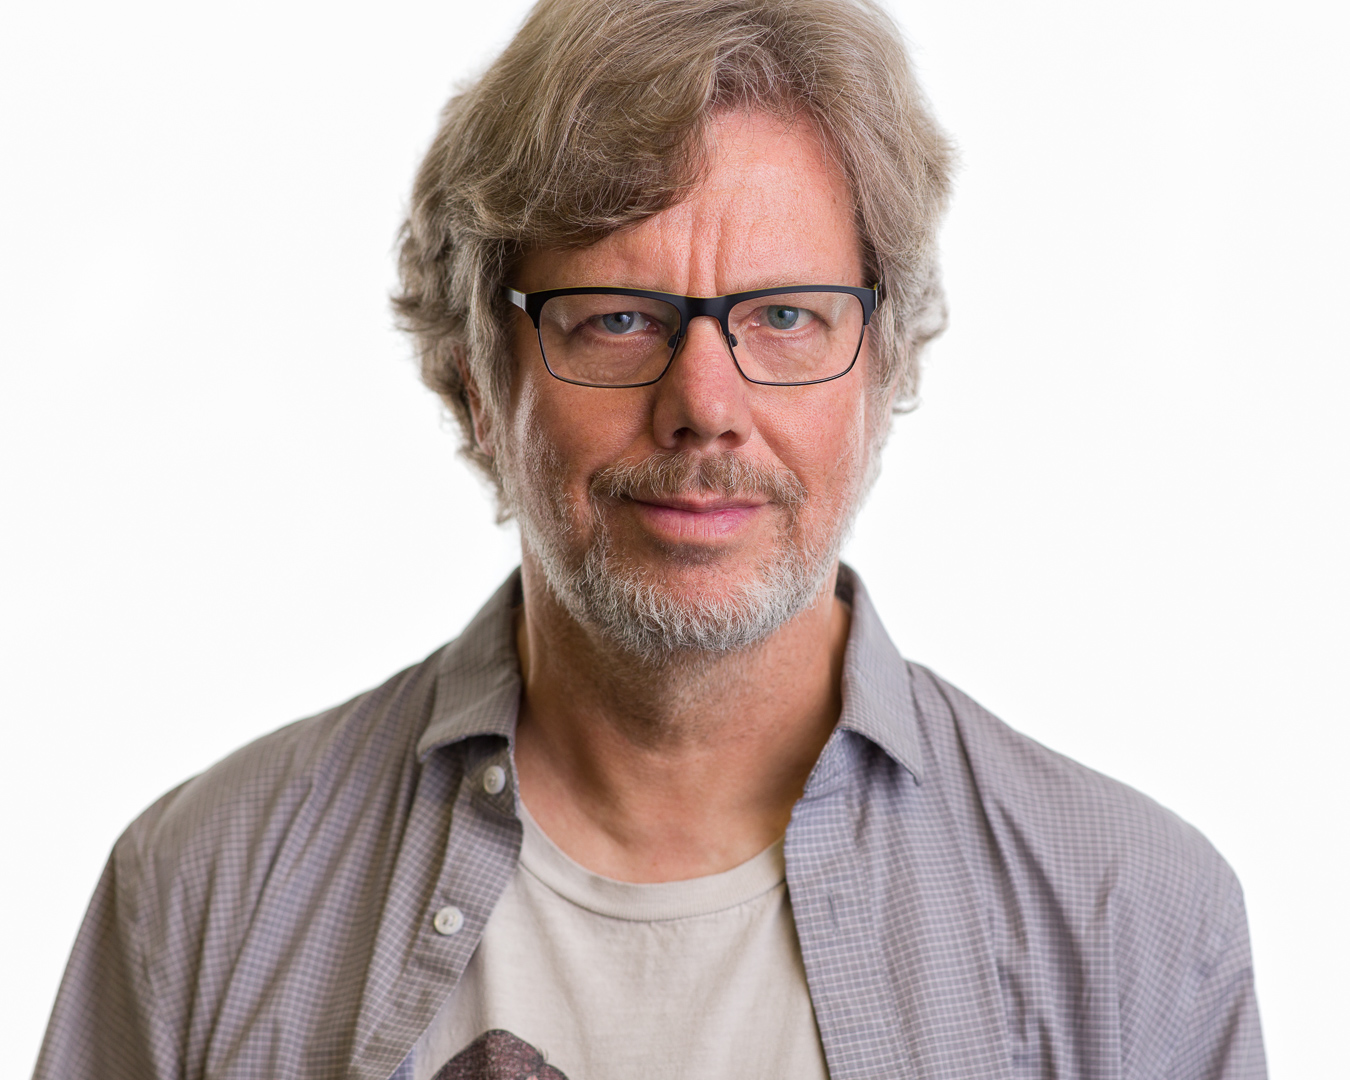
\includegraphics[scale=.5]{pics/guido-headshot-2019.jpg}
    \caption{Guido van Rossum}
    \label{fig:guido}
  \end{center}
\end{figure}

\section{Kenapa Python?}
Berikut adalah beberapa jawaban dari pertanyaan tersebut.
\begin{itemize}
  \item \textit{Multiplatform}. Python adalah bahasa pemrograman yang tersedia pada sejumlah \textit{platform} sistem operasi seperti \texttt{GNU Linux, Windows dan Mac}. Selain itu, Python juga tersedia pada \textit{platform} perangkat bergerak seperti Android dan \textit{embedded system}\footnote{\url{https://wiki.python.org/moin/EmbeddedPython}}.
  \item Mudah. Python merupakan bahasa pemrograman yang mudah karena \texttt{syntax} yang sederhana, sehingga mudah dikuasai bahkan oleh pengguna yang tidak memiliki latar belakang pendidikan formal di bidang ilmu komputer.
  \item Pustaka. Pustaka pendukung untuk banyak bidang ilmu tersedia secara bebas (bahkan terawat dengan baik oleh komunitas), terutama dalam keilmuan data di mana Python sangat populer saat ini \footnote{\url{https://towardsdatascience.com/top-9-languages-for-data-science-in-2020-824239f930c}}. Setidaknya, hal itu disebabkan oleh pustaka Python yang tersedia untuk tujuan \textit{data collection and cleansing}, \textit{data exploration}, \textit{data modeling} dan \textit{data visualization and interpretation} \footnote{\url{https://www.kdnuggets.com/2020/01/python-preferred-languages-data-science.html}}.
\end{itemize}

\section{Keilmuan data}
Keilmuan data secara umum didefinisikan sebagai metodologi yang darinya, \textit{actionable insight} dapat disimpulkan dari data sebagai dasar dalam pengambilan keputusan\cite{igual2017introduction}. Keilmuan data sangat multidisiplin dengan basis keilmuan utama ada pada ilmu komputer, statistik, dan domain ilmu lain yang menjadi obyek kajian\cite{skiena2017data} seperti ilustrasi di \figurename~\ref{fig:wordcloud}. Selain sifatnya sebagai keilmuan multidisiplin yang menjembatani teori, komputasi, eksperimen, dan \textit{biosocial area}, keilmuan data juga memerlukan interaksi dengan data dengan ukuran sangat besar, dinamis dan tidak selaras (\textit{incongruent})\cite{dinov2018data}. Karena itu, diperlukan algoritma, metode, \textit{tools} dan layanan yang mampu mengolah data tersebut dan menghasilkan sistem pendukung keputusan yang semi otomatis.

\begin{figure}
  \begin{center}
    \includegraphics{pics/wordcloud4datascience.png}
    \caption{\textit{Word cloud} untuk saling keterkaitan dalam keilmuan data \cite{braschler2019applied}}
    \label{fig:wordcloud}
  \end{center}
\end{figure}

Algoritma dan metode yang diperlukan untuk menghasilkan sistem pendukung keputusan saat ini banyak memanfaatkan pembelajaran mesin dan kecerdasan buatan, selain statistik sebagai pondasi keilmuannya. \figurename~\ref{fig:piramida} menunjukkan piramida di mana ilmuan data berperan\footnote{\url{https://towardsdatascience.com/data-engineer-vs-data-scientist-bc8dab5ac124}} dalam hirarki yang pertama kali dibuat oleh Monica Rogati\footnote{\url{https://medium.com/hackernoon/the-ai-hierarchy-of-needs-18f111fcc007}}. Berdasarkan hirarki tersebut, pelatihan ini mengasumsikan bahwa data telah tersedia (terutama dalam format CSV). Selanjutnya, peserta harus mampu berinteraksi dengan data tersebut, terutama untuk tujuan praproses sebelum nantinya diolah dengan algoritma tertentu memanfaatkan pustaka berbasis Python.

\begin{figure}
  \begin{center}
    \includegraphics[scale=.5]{pics/piramida.png}
    \caption{Hirarki kebutuhan kecerdasan buatan}
    \label{fig:piramida}
  \end{center}
\end{figure}

